

\documentclass{ocbeameruni}

\setdefaultlanguage[babelshorthands=true]{german}

\newcommand{\R}{\mathbb{R}}

\title{Organic Computing 2}
\subtitle{Lösungsvorschlag Blatt08}
\date{\today}
\author{Lukas Huhn \and Qiang Chang \and Victor Gerling}
\institute{%
  Universität Augsburg\\
  Institut für Informatik\\
  Lehrstuhl für Organic Computing
}

\usepackage{listings}

\begin{document}


\maketitle


\begin{frame}{Gliederung}
  \setbeamertemplate{section in toc}[sections numbered]
  \tableofcontents
\end{frame}


\section{Aufgabe 02}

\begin{frame}{2.1}
Implementieren Sie diesen und wenden Sie ihn auf das FrozenLake-v0-Szenario aus dem OpenAI-
Gym an!
    \begin{itemize}
    \item siehe Code.
    \end{itemize}
\end{frame}

\begin{frame}{2.2}
Finden Sie durch Ausprobieren oder eine kleine Parameterstudie geeignete Werte für die drei
Parameter ε, γ (Diskontierungsfaktor) und α (Lernrate)!
    \begin{itemize}
    \item alpha = 0.1
    \item gamma = 0.5
    \item epsilon = 0.09
    \end{itemize}
\end{frame}

\begin{frame}{2.2}
Zeichnen Sie ein Episode-Return-Diagramm sowie ein Episode-Returndurchschnitt-Diagramm,
wobei der Durchschnitt in Fenstern jeweils über die 100 Episoden vor der jeweiligen Episode
gebildet werden soll!
\end{frame}


\begin{frame}{2.3}
\begin{figure}[ht]
    \centering
    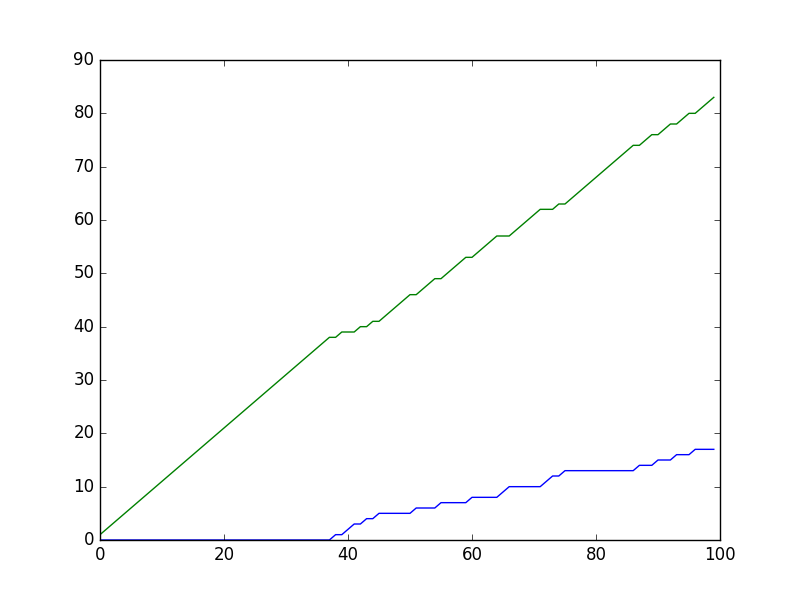
\includegraphics[width=50mm, height=50mm]{plots/figure_1.png} 
    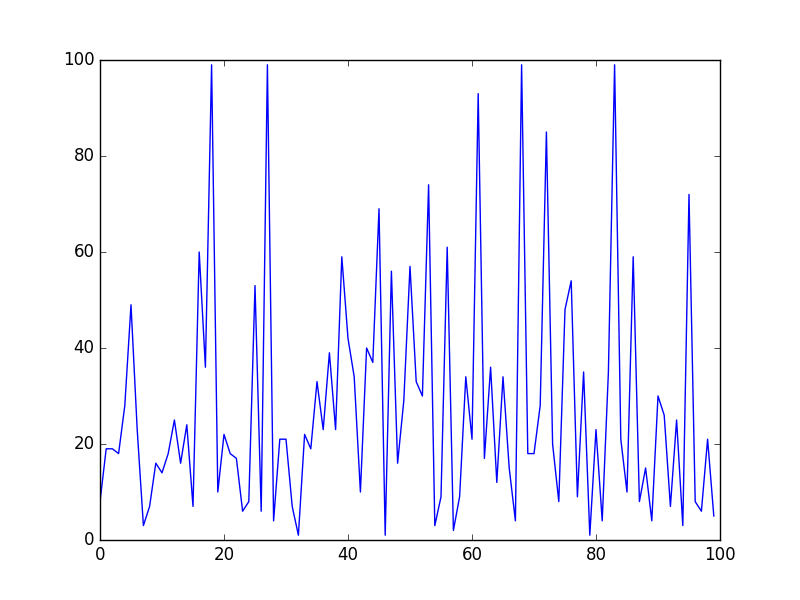
\includegraphics[width=50mm, height=50mm]{plots/figure_2.png} 
\end{figure}
 
\end{frame}


\begin{frame}[2.4]
Nach wie viel Episoden ist der Lernprozess zufriedenstellend abgeschlossen? Begründen Sie!
\begin{itemize}
\item Ein Versuch benötigte 452 Episoden um einen Gewinndurchschnitt von 0.51 zu erzielen.
\end{itemize}
\end{frame}


\begin{frame}[2.5]
Ist Q-Learning gut geeignet für dieses Szenario?
\begin{itemize}
\item Ja, da es einen diskreten Zustand- und Aktionsraum gibt, mit nur 16 möglichen Zuständen und 4 möglichen Aktionen.
Somit benötigen wir nur 16*4 = 64 q-Werte.
\end{itemize}
\end{frame}

\section{Aufgabe 03}

\begin{frame}[3.1]
Kann Ihre Q-Learning-Implementierung auch das CartPole-v1-Problem lösen? Wenn nicht:
Warum nicht?

Problem bei CarPole reicht der observation space
von
[-4.8000002e+00 -3.4028235e+38 -4.1887903e-01 -3.4028235e+38]
bis
[4.8000002e+00 3.4028235e+38 4.1887903e-01 3.4028235e+38]
\end{frame}

\begin{frame}[3.1]
1. Problem: Ist vier-dimensional. Lässt sich prinzipiell auf eine Array-Dimension reduzieren:
z.B. bei 8 Werten pro Richtung ergeben sich 8^4 states

2. Problem Werte sind nicht quantisiert. Es liegen zwischen -4 und 4 unendlich viele reale Werte. 
Lässt sich in Stufen aufteilen

    def quantize(val, min, max, levels):
      val = math.floor((val - min) * levels / (max - min))
      return val
\end{frame}


\begin{frame}[3.1]
3. Problem zweite und vierte Spalte reichen von -unendlich bis +unendlich, während beim Testen 
nur Werte nah an der null beobachtet werden konnten. Damit werden beide bei der Quantisierung
immer auf 0 abgebildetet also nicht vom Agenten wahrgenommen.
\end{frame}


\begin{frame}[3.2]
Wie könnte man Ihre Implementierung anpassen, um doch eine Lösung zu finden?

Für die Anpassung muss die Größe der q-Tabelle die Größe des quantisierten state-spaces haben,
in unserem Fall $(8^4)*2$, wobei 2 die Größe des Actionspaces bei Cartpole ist ({0, 1}).
\end{frame}

\begin{frame}[3.3]
Setzen Sie Ihre Idee um. Funktioniert sie? Weshalb (nicht)? Wie lange dauert der Lernprozess?

Es wurde mit 4096 * 4 * 10 Iterationen Gelernte, sodass jedes gültige 
State-Action-Paar durchschnittlich 10 mal besucht werden konnte. Das Ergebnis ist ernüchternt, der Agent
hält das Gleichgewicht keine Sekunde.

Die liegt vermutlich an den nicht-wahrgenommen Zustands-Attributen.

Vielleicht kann wäre auch eine andere Form der Generalisierung für die reelwertigen Attribute günstiger.
\end{frame}

\end{document}
% Local Variables:
% TeX-engine: xetex
% End:
